\documentclass[../main.tex]{subfiles}
\begin{document}


\section{Neuronale Netze}

\begin{figure}[h!]
  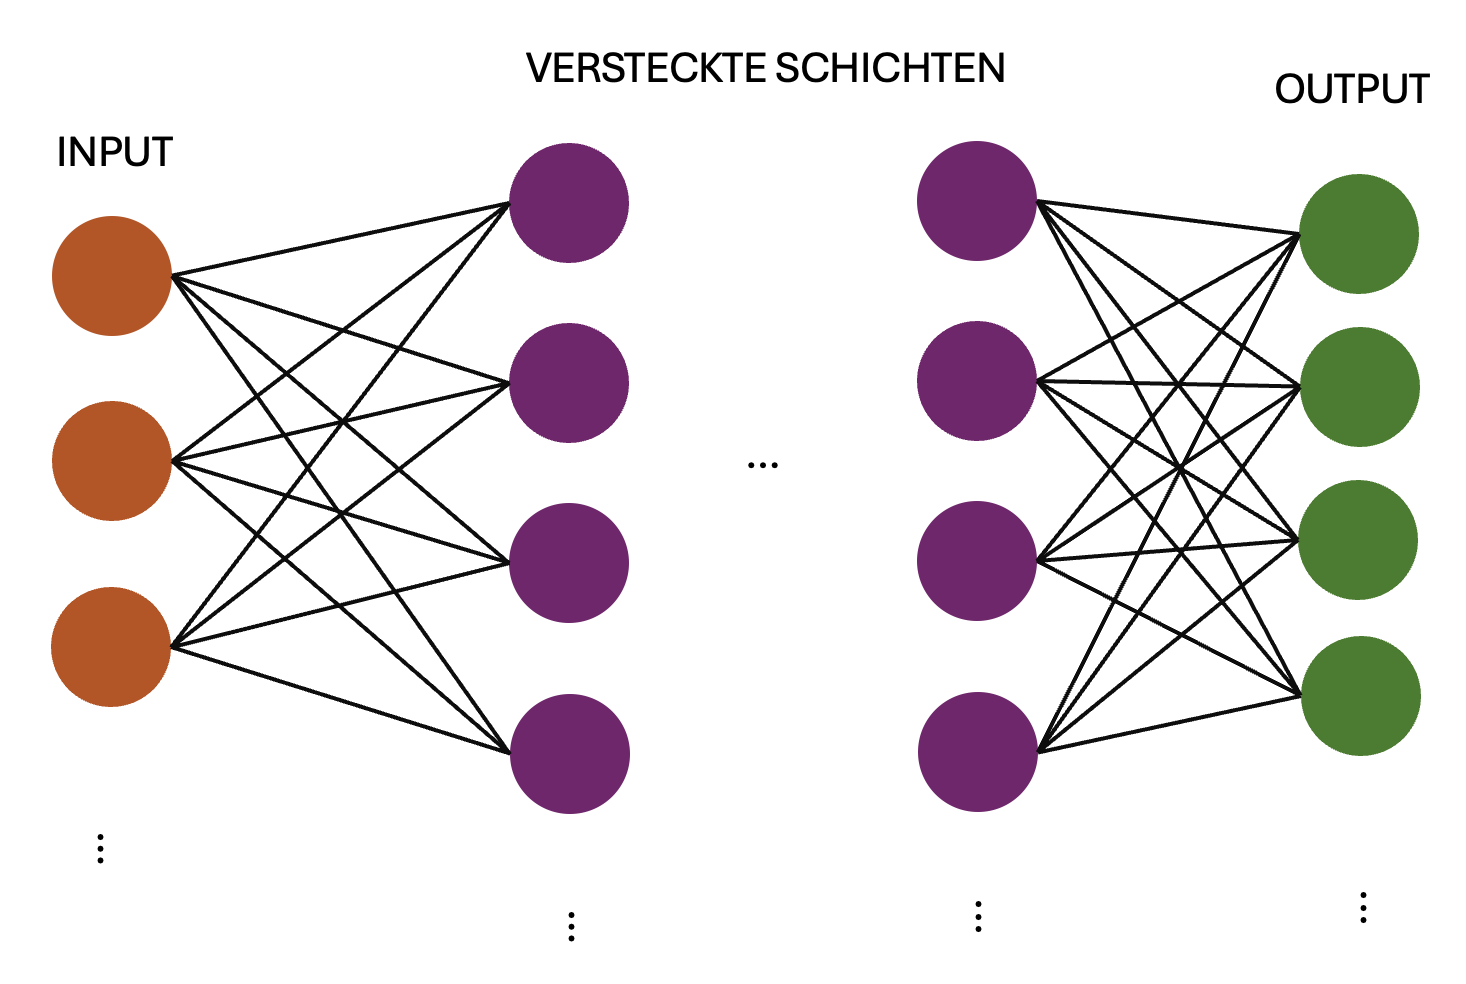
\includegraphics[scale=0.6]{bilder/NeuralNetwork.png}
  \caption{Neuronales Netzwerk}
  \label{fig:NN}
\end{figure}

\glspl{nn} bilden die Basis für \glslink{glos:ki}{KI} und sind in ihrer Funktionsweise dem menschlichen Gehirn nachempfunden. Sie bestehen aus einer Anzahl von Neuronen, die – wie in Abb. \ref{fig:NN} dargestellt – in verschiedenen Schichten angeordnet sind. Die erste Schicht heißt Eingabeschicht, die letzte Ausgabeschicht, dazwischen liegen sogenannte versteckte Schichten. Jedes Neuron ist über gewichtete Verbindungen mit allen Neuronen der vorherigen und nachfolgenden Schicht verbunden. Ein Neuron nimmt zu jedem Zeitpunkt einen Wert zwischen 0 und 1 an, welcher dem Output des Neurons entspricht. Dieser Wert wird aus der Verarbeitung der Inputs errechnet, also aus den Outputs der vorherigen Schicht, auf deren Summe eine Funktion angewandt wird. \\
Jede Verbindung zwischen Neuronen verfügt über eine Gewichtung zwischen -1 und 1, die bestimmt, mit welcher Zahl der Wert eines Neurons multipliziert wird, bevor er an die nächste Schicht weitergegeben wird. Die Gewichtungen zwischen zwei Schichten können als Matrix dargestellt werden, und der Übergang zwischen Schichten entspricht einer Matrixmultiplikation. \\
Die Gewichtungen stehen zu Beginn noch nicht fest, sondern werden durch das Training bestimmt. Das Training eines \glslink{glos:nn}{NN} ist die Anpassung dieser Gewichtungen mittels Backpropagation. Dazu werden die Gewichtungen zunächst zufällig gewählt und das \glslink{glos:nn}{NN} durchläuft viele Trainingsdaten. Die erhaltenen Ergebnisse werden mit den gewünschten verglichen. Bei zu großen Abweichungen werden alle zugehörigen Gewichtungen reduziert, bei Übereinstimmung werden sie erhöht. \glslink{glos:nn}{NN}s sind die Grundlage für Technologien wie \glspl{llm}, die auch für \glslink{glos:ki}{KI}-Schreibwerkzeuge verwendet werden. 

\section{Large Language Models}
\label{sec:llm}

\begin{figure}[h!]
  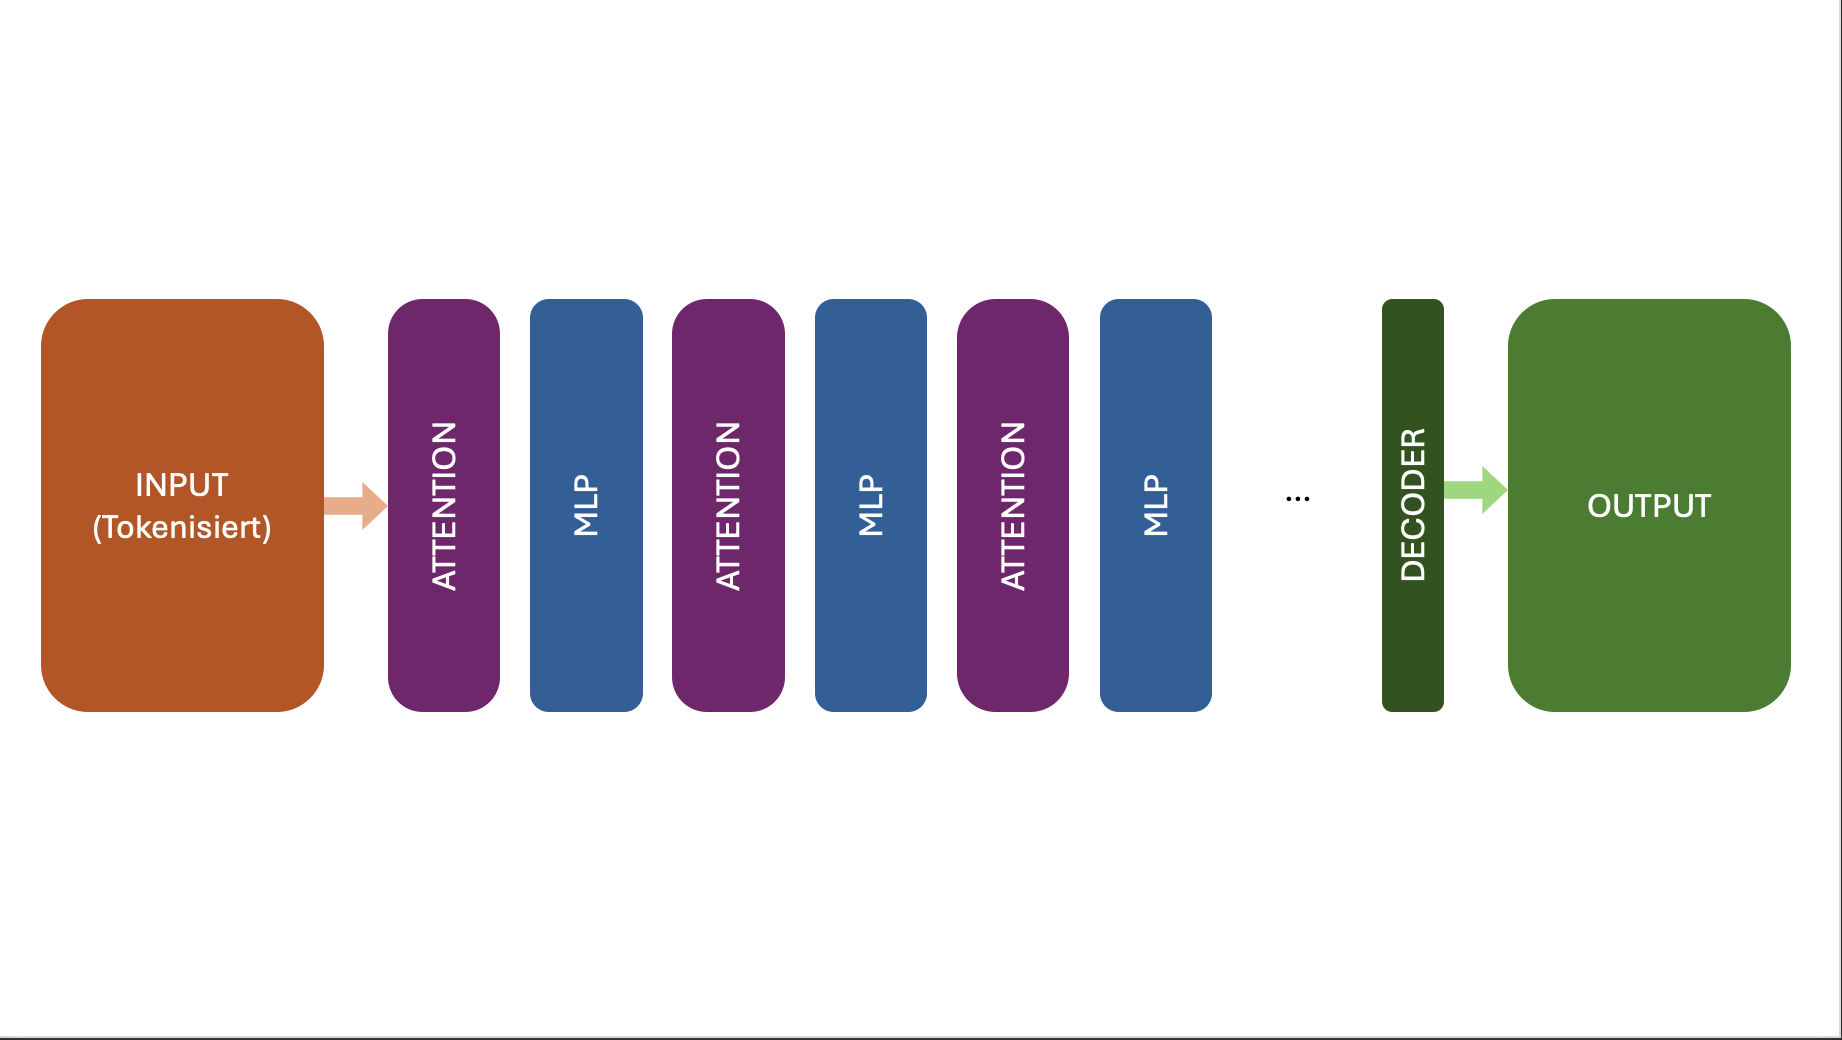
\includegraphics[scale=0.37]{bilder/Transformer.png}
  \caption{Transformer}
  \label{fig:trans}
\end{figure}

\glspl{llm} sind eine Form der \glslink{glos:ki}{KI}, die auf natürlicher Sprache basiert. Da sie entwickelt wurden, um Texte zu generieren, werden \glspl{llm} als generative 
\glslink{glos:ki}{KI} bezeichnet. Moderne \glslink{glos:llm}{LLM}s wie ChatGPT basieren auf einer Transformer-Architektur, die in Abb. \ref{fig:trans} schematisch dargestellt ist. Diese 
berechnet aus einem Eingabetext eine Wahrscheinlichkeitsverteilung über mögliche nächste Tokens. Die Transformerarchitektur besteht aus folgenden Komponenten:\cite{architecture}\\

\begin{itemize}

\item \textbf{Tokenisierung:} Zuerst wird der Eingabetext in Tokens unterteilt. Tokens können Wörter, Wortteile, Satzzeichen oder einzelne Buchstaben sein. Sie sind die kleinste Einheit, 
die das \glslink{glos:llm}{LLM} verarbeiten kann.\cite{architecture}

\item \textbf{Embedding:} Tokens werden vieldimensionalen Vektoren zugeordnet. So werden sie anhand ihrer Bedeutung codiert. Die Richtungen der Vektoren im
Vektorraum beinhalten semantische Bedeutungen. Wörter mit ähnlicher Bedeutung liegen als Vektoren im Vektorraum nahe beieinander.\cite{embedding}

\item \textbf{Attention:} Die vektorcodierten Tokens werden durch den umliegenden Text verändert, um den Wortkontext und die semantische Bedeutung widerzuspiegeln.\\
Ein Beispiel: In den Sätzen "`Ich sitze auf der Bank"' und "`Ich habe in der Bank Geld abgehoben"' erhält "`Bank"' jeweils eine andere Vektorrepräsentation, je nach Kontext liegen die codierenden 
Vektoren nahe der Tokens "`Parkbank"' oder "`Kreditinstitut"'. So bleibt der Kontext des verwendeten Wortes erhalten.\cite{attention, attention2} 

\item \textbf{\acrfull{mlp}:} Neben der linearen Attention-Funktion können mit dem \acrshort{mlp}, einem kleinen neuronalen Netzwerk mit meist nur einer inneren Schicht, auch nichtlineare Zusammenhänge 
erfasst werden. Jeder Vektor durchläuft das \acrshort{mlp}, dessen Ausgabe zum ursprünglichen Vektor addiert wird. Somit kann die Komplexität der Sprache erfasst werden.

\item \textbf{Decoder:} Ein \glslink{glos:llm}{LLM} besteht aus abwechselnden Attention- und MLP-Schichten (Abb. \ref{fig:trans}). Abschließend erhält der Decoder die Ausgabe aus der letzten 
\acrshort{mlp}-Schicht, worauf die Softmax-Funktion eine Wahrscheinlichkeitsverteilung über alle Tokens berechnet. Durch die Anwendung dieser Funktion ist die Summe der Wahrscheinlichkeiten 1 und jede liegt im Intervall zwischen 0 und 1.\cite{architecture} 
\end{itemize}

Basierend auf der sich so ergebenen Wahrscheinlichkeitsverteilung wählt das \glslink{glos:llm}{LLM} zufällig ein nächstes Wort und fügt es dem Text an. Der Vorgang wiederholt sich mit dem aktualisierten Text, 
bis eine Abbruchbedingung eintritt, etwa eine maximale Tokenanzahl oder ein spezielles Abbruchtoken.\cite{architecture}\\

\section{\gls{glos:prompt} und Kontext}

Um nun zu bestimmen, was für einen Text das \glslink{glos:llm}{LLM} generieren soll, erhält es einen Input. Dieser wird als \gls{glos:prompt} bezeichnet. Da \glslink{glos:ki}{KI}-Modelle verschiedene Prompts bearbeiten können, ist es 
möglich, ein Modell zum Lösen unterschiedlichster Aufgaben einzusetzen. Der Prompt setzt sich aus dem System-Prompt sowie dem User-Prompt zusammen. Zudem können noch weiteren Kontext-Angaben 
ergänzt werden.\cite{systemprompt}\\
Der System-Prompt stellt die Grundstruktur des Prompts dar und gibt dem \glslink{glos:llm}{LLM} einen grundlegenden Kontext für die Generierung des Textes mit. Zuerst wird die Information mitgeteilt, dass eine 
Frage beantwortet beziehungsweise auf eine Nutzereingabe reagiert werden soll. Darüber hinaus wird dem Modell mitgeteilt, dass es im folgenden Chat die Rolle des \glslink{glos:ki}{KI}-Assistenten übernimmt. 
Meistens werden im System-Prompt noch weitere Informationen mitgegeben, wie zum Beispiel der Stil oder Ton des Textes. Außerdem kann dem \glslink{glos:llm}{LLM} hier mitgeteilt werden, dass bestimmte Wörter 
nicht benutzt oder bestimmte Themen nicht angesprochen werden sollen, also eine erste Stufe von Filtern eingebaut werden.\cite{systemprompt}\\
Der System-Prompt wird meist durch die Entwickler des \glslink{glos:llm}{LLM}s festgelegt und ändert sich nicht. Deswegen wird er auch als "`Fixed-Prompt"' bezeichnet. Er ist für den Nutzer meist nicht sichtbar.\\
Der zweite Bestandteil des Prompts ist der User-Prompt, welcher konkret vom Nutzer eingegeben wird. Dieser kann sich bei jeder neuen Anfrage ändern und ist für den Nutzer nicht nur sichtbar, sondern 
auch veränderbar. Verändert man den Prompt, um ein besseres oder passenderes Ergebnis zu erzielen, wird dies als Prompt-Engineering bezeichnet. Um den Prompt effektiv anpassen zu können, um 
ein gewünschtes Ergebnis zu erreichen, sind oft viele Versuche nötig sowie ein tief gehendes Verständnis für die Funktionsweise des \glslink{glos:llm}{LLM}s.\cite{promptengineering}\\
Zusätzlich zum System-Prompt und User-Prompt können dem \glslink{glos:llm}{LLM} noch mehr Informationen mitgegeben werden. Die Summe aus dem Prompt und weiteren Angaben wird als Kontext bezeichnet. Dazu zählen 
zum Beispiel der vorherige Chatverlauf, damit das \glslink{glos:llm}{LLM} sich auf die vorherige Konversation beziehen kann. Auch Texte, die für die Generierung der Antwort relevant sind, können im Kontext 
übergeben werden. Ein weiteres Beispiel ist das sogenannte Few-Shot-Learning, bei dem eine  beispielhafte Konversation zwischen dem Nutzer und dem \glslink{glos:llm}{LLM} dargestellt wird, um Beispiele für das 
gewünschte Format oder den Stil der Antwort zu geben.\cite{kontext,FewShot}\\
Das Kontextfenster bezeichnet die maximale Anzahl an Tokens, die dem \glslink{glos:llm}{LLM} als Input mitgegeben werden können. Wird diese Anzahl überschritten, wird der Inhalt nicht vollständig mitgegeben, 
was zu ungewünschten und unvollständigen Ergebnissen führen kann.

\section{Wirkungen und Nebenrisiken}
Mit dieser Architektur entstehen Texte, die menschengeschriebenen stark ähneln und zahlreiche Anwendungsgebiete eröffnen. Gleichzeitig ergeben sich daraus auch Herausforderungen und Risiken, 
die im Folgenden behandelt werden.

\subsection{Abhängigkeit von den Trainingsdaten}

Da \glslink{glos:ki}{KI} Zusammenhänge lediglich auf Grundlage der verwendeten Trainingsdaten erlernt, sind diese häufig die Ursache für Probleme. Werden beispielsweise Trainingsdaten verwendet, 
bei denen bestimmte Personengruppen benachteiligt werden oder seltener Vorkommen, kann das die generierten Inhalte der \glslink{glos:ki}{KI} beeinflussen. Diskriminierende Inhalte können aus den Trainingsdaten 
übernommen werden. Zudem können sich durch fehlende Informationen über bestimmte Personengruppen, Sprachen, Dialekte etc. auch Nachteile in der Nutzung von \glslink{glos:ki}{KI} für betroffene 
Personengruppen ergeben.\\ Dieses Verhalten generativer \glslink{glos:ki}{KI} kann sowohl soziale als auch wirtschaftliche Folgen haben. \glslink{glos:ki}{KI} Anbieter versuchen zwar, diesem Problem durch eine möglichst 
facettenreiche Auswahl von Trainingsdaten und dem Einbau von Filtern, welche beispielsweise das Auftreten bestimmter Wörter wie Beleidigungen verhindern, diesem Problem entgegenzuwirken, 
dennoch sollten sich Nutzer diesem Risiko bewusst sein.\\

\subsection{Halluzinationen}

Die Texte, welche eine \glslink{glos:ki}{KI} ausgibt, können falsche Informationen beinhalten. Diese werden häufig als "`Halluzinationen"' bezeichnet. \glslink{glos:ki}{KI}-Halluzination beschreibt 
das Phänomen, dass generative \glslink{glos:ki}{KI}-Anwendungen Antworten erzeugen, welche zwar plausibel erscheinen, jedoch in Wirklichkeit unlogisch oder unzutreffend sind\cite{hallucinationForewarning}.\\
Halluzinationen können verschiedene Ursachen haben. Auch dafür bilden Probleme mit den Trainingsdateninhalten einen potentiellen Grund. Sind die Trainingsdaten schon älter,
können sie veraltete Informationen enthalten. Durch das Fehlen aktueller Daten kann das \glslink{glos:ki}{KI}-Modell keine korrekten Aussagen zu aktuellen Ereignissen tätigen.\\ Des 
Weiteren können die Daten ungenau, nicht fallspezifisch oder inkorrekt sein. Besonders bei einem Modelltraining mit Daten aus dem Internet besteht die Gefahr, dass 
Trainingsdaten Fehler enthalten.\\ Als weitere potenzielle Ursache für Halluzinationen kommen Schwachstellen in der Architektur in Betracht. Als "`Sycophancy"' wird das 
Phänomen beschrieben, dass das \glslink{glos:ki}{KI}-Modell Texte generiert, welche den Erwartungen des Nutzers entsprechen, ohne dabei auf fachliche Korrektheit zu achten. Dies kann ebenfalls 
durch die Formulierung des \gls{glos:prompt}s beeinflusst werden.\cite{allgemHalluzinationen} \\
Ferner birgt die Methode, mit welcher \glslink{glos:ki}{KI} Texte generiert, ein Risiko für Falschinformationen. Beispielsweise wird durch eine hohe Temperatureinstellung die 
Wahrscheinlichkeit für unplausible oder falsche Inhalte größer. Ein Artikel der Frauenhofer-Institutes beschreibt, dass gewisse Token-Typen sehr nah beieinander liegen 
und somit auch ähnliche Wahrscheinlichkeiten haben. Dazu zählten zum Beispiel "`ähnliche numerische Werte wie Preise (9,99 EUR; 10,00 EUR), nahe beieinander liegende 
Daten (2020, 2021), ähnlich klingende Namen, oder technische Begriffe und Abkürzungen (\glslink{glos:ki}{KI}, ML)"'\cite{halluzinationenFraunhofer}. Eine Verwechslung dieser Daten kann ebenfalls zu inkorrekten Aussagen 
führen.\\
Darüber hinaus können bei der Auswahl des nächsten Tokens aufgrund der Wahrscheinlichkeit, wie in \autoref{sec:llm}  beschrieben, unpassende Wörter bevorzugt werden, welche 
daraufhin die Grundlage für Halluzinationen bilden. Technisch begründet ist dieses Phänomen mit dem sogenannten Softmax-Bottleneck. Bei der Generierung der Liste von 
Wahrscheinlichkeiten für das nächste Wort wird der Softmax-Algorithmus auf einen mehrdimensionalen Vektor angewendet. Aufgrund der Natur dieses Algorithmus kann nur 
ein Ausschnitt aller möglichen Wahrscheinlichkeitsverteilungen dargestellt werden. Dadurch kann es passieren, dass die Verteilung nicht korrekt abgebildet und 
unpassenden Wörtern eine höhere Wahrscheinlichkeit zugeschrieben wird.\cite{softmax} \\
Ein so gewähltes unpassendes Wort, welches dem Text angefügt wird, bildet wiederum die Grundlage für das Generieren der darauffolgenden Wörter. Sobald in einem \glslink{glos:ki}{KI}-Chat eine 
bestimmte Falschinformation auftritt, kann die sogenannte "`Over-Confidence"' dazu führen, dass auch bei wiederholtem Nachfragen oder versuchtem Korrigieren der 
Aussage, das \glslink{glos:ki}{KI}-Modell weiterhin auf die Korrektheit der Behauptungen besteht. Dies erschwert das Überprüfen der Fakten für den Anwender.\cite{allgemHalluzinationen,softmax} \\
Selbst wenn ein \glslink{glos:ki}{KI}-generierter Text keine Falschinformationen enthält, können die beschriebenen Phänomene eine Unvollständigkeit der generierten Texte hervorrufen 
oder zu einem Abweichen von der eigentlichen Fragestellung führen.  Das als "`Instructions-Forgetting"' bekannte Phänomen beschreibt, dass eine \glslink{glos:ki}{KI} den Kontext der 
ursprünglichen Anfrage vergisst und einen Text generiert, der inhaltlich nicht der Fragestellung entspricht. Deswegen sollten \glslink{glos:ki}{KI}-generierte Texte, besonders im Kontext 
des wissenschaftlichen Schreibens, immer überprüft werden.\cite{allgemHalluzinationen}


\subsection{Erklärbarkeitsproblem}
\label{sec:erklärbarkeitsproblem}

Das Erklärbarkeitsproblem adressiert die Schwierigkeit, die Begründung für spezifische Entscheidungen \glslink{glos:ki}{KI} nachvollziehbar zu machen. Aufgrund der Funktionsweise nach dem sogenannten 
"`Black-Box"'-Prinzip ist die Rekonstruktion der kausalen Faktoren, die zu einem bestimmten Ergebnis geführt haben, limitiert. Diese Intransparenz kann die Akzeptanz und das Vertrauen in 
KI-basierte Entscheidungen beeinträchtigen. Darüber hinaus erschwert sie die Identifizierung und Korrektur von Fehlern in der zugrundeliegenden Architektur. Aktuelle Forschungsansätze 
im Bereich der "`erklärbaren KI"' zielen darauf ab, dieses Problem zu adressieren, indem sie beispielsweise Mechanismen zur Visualisierung und Darstellung des 
Entscheidungsfindungsprozesses entwickeln.\cite{explainable}
 

\subsection{Ressourcenverbrauch}

KI-Modelle verbrauchen sowohl während des Trainings als auch beim Bearbeiten der Anfragen viele Ressourcen. Desto größer das verwendete Modell, desto höher ist auch der Ressourcenverbrauch. 
Der Stromverbrauch von GPT4 0.1 liegt laut eines im Jahr 2025 veröffentlichten Artikels bei bis zu einer Kilowattstunde pro Anfrage\cite{Energieverbrauch}. Für die oben beschriebene Anpassung der Parameter sind während des Bearbeitens einer Anfrage viele 
komplexe Berechnungen in möglichst kurzer Zeit notwendig. Auch das Training ist durch die große Menge benötigter Daten und die häufig wochen- bis monatelangen Trainingszeiten 
energieintensiv. In den Rechenzentren wird zudem Wasser zur Kühlung verwendet. Der Wasser-und Ressourcenverbrauch der Nutzung eines \glslink{glos:ki}{KI}-Modells ist im Vergleich zu dem der Nutzung einer 
Suchmaschine wie Google sehr hoch\cite{KINachhaltigkeit}. 

\subsection{Datenschutz}
\label{sec:datenschutz}

Zudem besteht beim Training sowie bei der Nutzung von \glslink{glos:ki}{KI} das Problem des Datenschutzes. Die Trainingsdaten können personenbezogene Daten beinhalten. Das \glslink{glos:ki}{KI}-Modell kann bestimmte sensible 
Informationen aus den Trainingsinhalten wiedergeben, auch wenn diese nicht absichtlich gespeichert werden sollen. Einige \glslink{glos:llm}{LLM}-Anbieter behalten sich das Recht vor, das Modell anhand der 
Eingabedaten weiter zu trainieren und die Daten anderweitig zu nutzen. Auch so können personenbezogenen oder unternehmensspezifischen Informationen in die Trainings- oder Ausgabedaten 
erscheinen und so zu Datenschutzverletzungen führen. Im Falle einer missbräuchlichen Verwendung solcher Daten ist oft unklar, wer dafür die Verantwortung trägt. Vor allem bei der \glslink{glos:ki}{KI}-Nutzung 
über Online-Schnittstellen sollte daher sorgfältig mit wichtigen Informationen umgegangen werden. Sie sollten beispielsweise nicht in Form des \gls{glos:prompt}s an das Modell gegeben werden.

\end{document}